\documentclass[journal]{new-aiaa}

\usepackage[utf8]{inputenc}
\usepackage{textcomp}
\usepackage{graphicx}
\usepackage{amsmath}
\usepackage{siunitx}
\usepackage{booktabs}
\usepackage{longtable,tabularx}
\setlength\LTleft{0pt}

\title{Preliminary Progress Report: Adaptive Physics-Informed Thermal Monitoring of a Rocket Throat Wall}

\author{Gabriel Berezovsky}
\affil{gabrielb@campus.technion.ac.il, 941220121}
\author{Joshua Blecher}
\affil{bjoshua@campus.technion.ac.il, 941220097}
\author{Nathan Florsheim}
\affil{nathanf@campus.technion.ac.il, 800001653}

\begin{document}

\maketitle

\begin{abstract}
This preliminary report describes a feasible physics-informed machine-learning project for transient thermal monitoring of a regeneratively cooled rocket-engine throat wall. The full rocket engine problem is intentionally reduced to one-dimensional heat conduction through the wall thickness. A finite-difference Crank--Nicolson solver generates a trusted synthetic reference solution. A baseline physics-informed neural network (PINN) is then trained to satisfy the heat equation, boundary conditions, and initial condition. Our controlled modification is an adaptive PINN: after baseline training, sparse thermocouple-like measurements are revealed in time windows and used to fine-tune the same model. Preliminary three-seed results show that adaptive sensor assimilation reduces the global relative $L_2$ error from $0.1312 \pm 0.0019$ to $0.0689 \pm 0.0045$ and reduces the hot-side maximum temperature error from $27.53 \pm 0.19$ K to $16.56 \pm 0.49$ K.
\end{abstract}

\section*{Nomenclature}
{\renewcommand\arraystretch{1.0}
\noindent\begin{longtable*}{@{}l @{\quad=\quad} l@{}}
$c_p$ & wall specific heat capacity, J/(kg K)\\
$h_{\mathrm{cool}}$ & coolant-side heat-transfer coefficient, W/(m$^2$ K)\\
$k$ & wall thermal conductivity, W/(m K)\\
$L$ & wall thickness, m\\
$q_{\mathrm{hot}}(t)$ & imposed hot-gas-side heat flux, W/m$^2$\\
$T(x,t)$ & wall temperature, K\\
$T_{\mathrm{cool}}$ & coolant reference temperature, K\\
$T_0$ & initial wall temperature, K\\
$x$ & coordinate through the wall thickness, m\\
$\alpha$ & thermal diffusivity, $k/(\rho c_p)$, m$^2$/s\\
$\Delta T$ & reference temperature scale used for nondimensionalization, K\\
$\theta$ & nondimensional temperature rise, $(T-T_{\mathrm{cool}})/\Delta T$\\
$\rho$ & wall density, kg/m$^3$\\
\end{longtable*}}
\addtocounter{table}{-1}

\section{Physical Problem and Simplifying Assumptions}
The original engineering motivation is real-time thermal monitoring of a rocket-engine throat wall. This region is exposed to large hot-gas heat flux on the inner wall and active regenerative cooling on the other side, a standard concern in rocket thermal design \cite{oates1984aerothermodynamics}. Modeling the full problem would require combustion, turbulent flow, coolant-channel geometry, and coupled fluid--solid heat transfer. That is too large for the current project. Instead, we keep the thermal-monitoring idea but reduce the geometry to a one-dimensional wall slab, shown schematically in Fig.~\ref{fig:setup}.

\begin{figure}[h!]
    \centering
    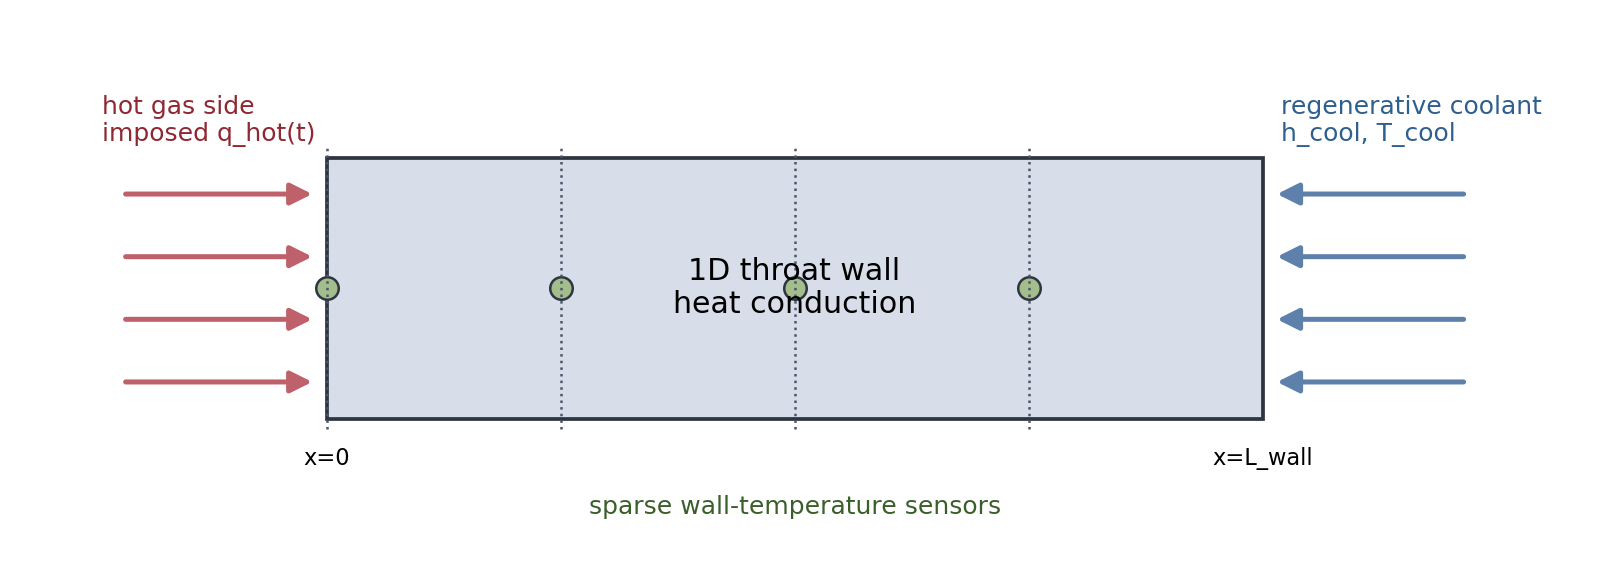
\includegraphics[width=0.95\linewidth]{figures/physical_setup.png}
    \caption{Reduced physical system. The coordinate $x=0$ is the hot-gas side and $x=L$ is the coolant side. Sparse sensor locations are treated as thermocouple-like wall-temperature observations.}
    \label{fig:setup}
\end{figure}

The assumptions for the preliminary model are:
\begin{itemize}
    \item one-dimensional heat conduction through the wall thickness;
    \item constant copper-like wall properties $(\rho,c_p,k)$;
    \item no internal heat generation;
    \item a prescribed, smooth hot-side heat flux $q_{\mathrm{hot}}(t)$;
    \item a Robin convection condition on the coolant side;
    \item synthetic thermocouple data generated from the finite-difference reference solution.
\end{itemize}

The governing equation is the transient heat equation
\begin{equation}
\rho c_p \frac{\partial T}{\partial t}
= k \frac{\partial^2 T}{\partial x^2},
\qquad 0 \le x \le L,\; 0 \le t \le t_f .
\label{eq:heat_dimensional}
\end{equation}
The boundary and initial conditions are
\begin{align}
-k \frac{\partial T}{\partial x}(0,t) &= q_{\mathrm{hot}}(t), \label{eq:hot_bc}\\
-k \frac{\partial T}{\partial x}(L,t) &= h_{\mathrm{cool}}\left(T(L,t)-T_{\mathrm{cool}}\right), \label{eq:cool_bc}\\
T(x,0) &= T_0. \label{eq:ic}
\end{align}
Figure~\ref{fig:forcing} shows the imposed heat flux and the resulting reference hot- and coolant-side temperatures.

\begin{figure}[h!]
    \centering
    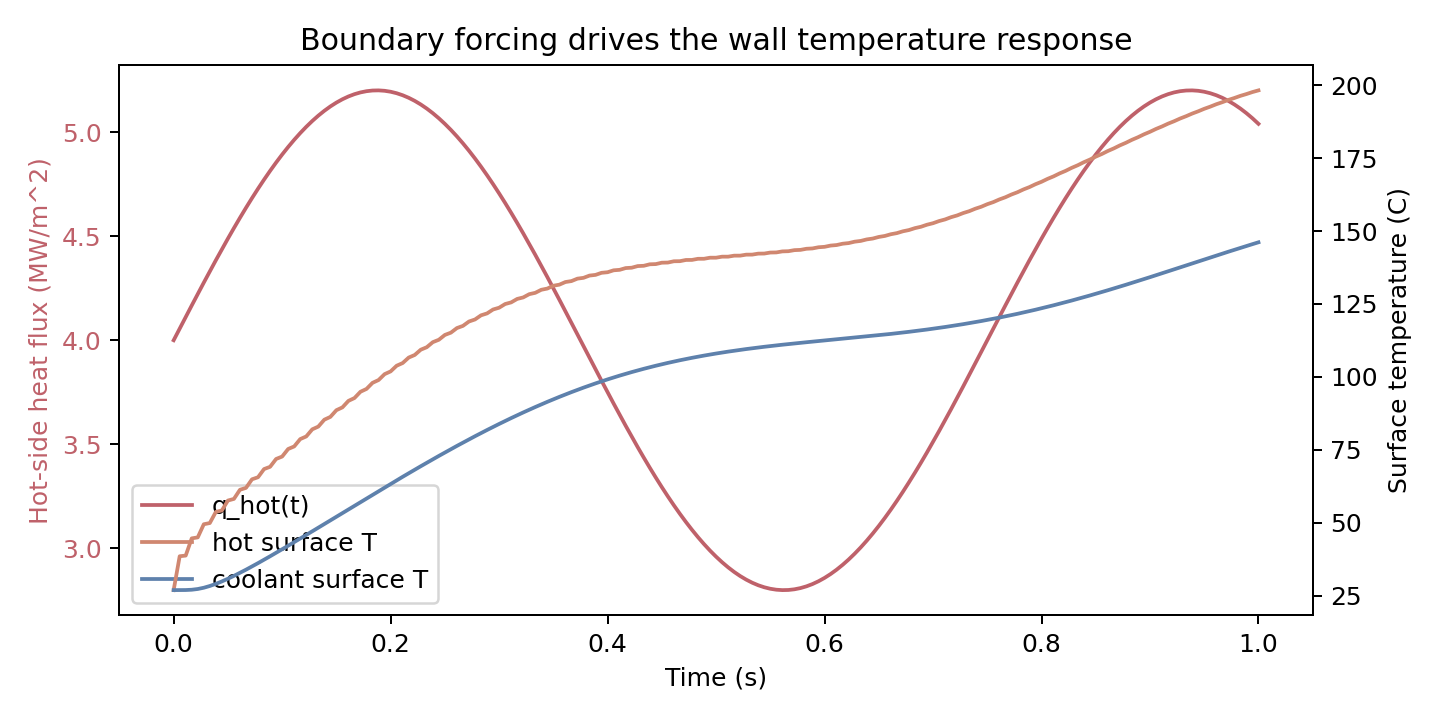
\includegraphics[width=0.82\linewidth]{figures/boundary_forcing_and_surfaces.png}
    \caption{The hot-side boundary is driven by a smooth imposed heat flux. The finite-difference reference solution responds with a larger temperature rise on the hot side and a smaller delayed response near the coolant side.}
    \label{fig:forcing}
\end{figure}

\section{Where the Data Comes From}
No experimental rocket data is used at this stage. All data is synthetic and reproducible. First, Eq.~\eqref{eq:heat_dimensional}--\eqref{eq:ic} is solved numerically using a Crank--Nicolson finite-difference method, a standard implicit approach for transient heat-transfer problems \cite{patankar1980numerical}. Crank--Nicolson averages the heat equation between time levels $n$ and $n+1$. For a linear heat equation, this gives a stable reference solution without requiring a very small time step.

In simple terms, the finite-difference grid stores temperatures $T_i^n \approx T(x_i,t_n)$. At each new time step, the method solves a tridiagonal-like linear system for the next temperature profile. This produces the full temperature field shown in Fig.~\ref{fig:reference}. We then sample this field at a few fixed wall locations to create sparse thermocouple-like measurements. These measurements are not independent training data from an experiment; they are withheld samples from the reference solution, optionally with noise added.

\begin{figure}[h!]
    \centering
    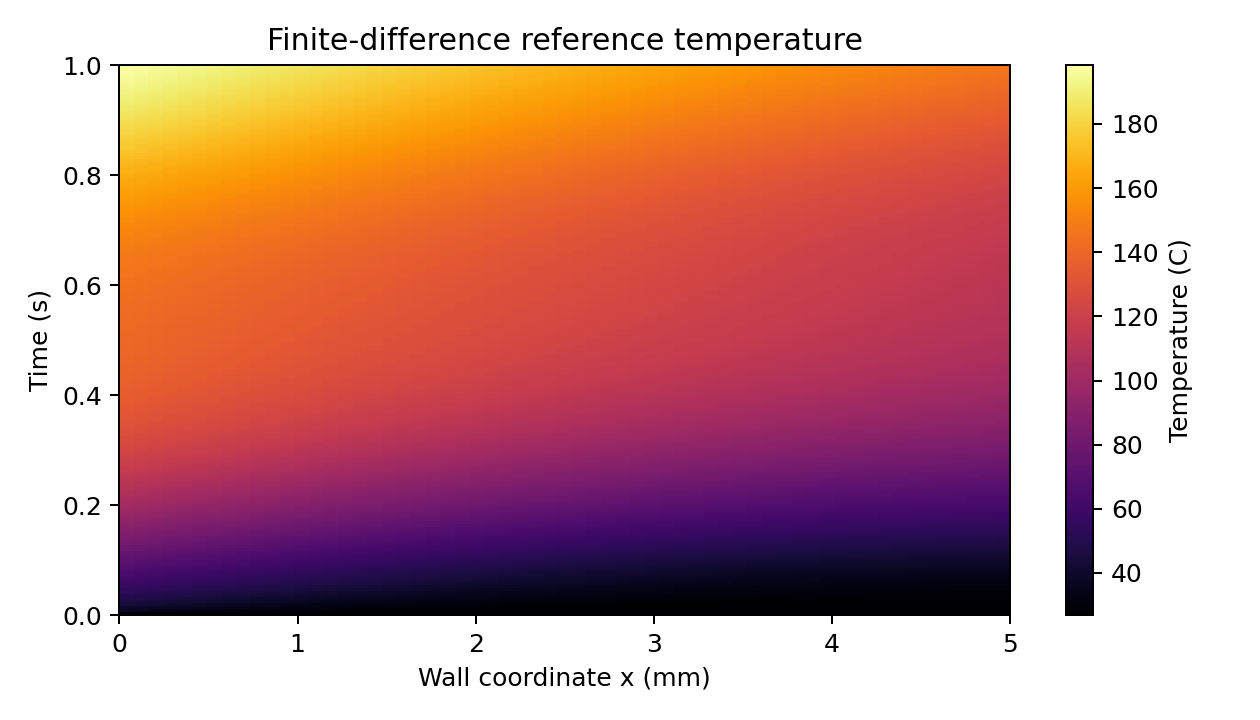
\includegraphics[width=0.82\linewidth]{figures/reference_temperature_field.png}
    \caption{Finite-difference reference solution used as synthetic ground truth. This is the solution against which the PINN predictions are evaluated.}
    \label{fig:reference}
\end{figure}

\section{PINN Design and Training}
The neural network is a small fully connected PyTorch model. Its inputs are nondimensional space and time,
\begin{equation}
\hat{x} = \frac{x}{L}, \qquad \hat{t} = \frac{t}{t_f},
\end{equation}
and its output is nondimensional temperature rise,
\begin{equation}
\theta(\hat{x},\hat{t}) = \frac{T(x,t)-T_{\mathrm{cool}}}{\Delta T}.
\end{equation}
This scaling keeps the network inputs and outputs near order one.

The baseline PINN is trained without sensor data, following the standard physics-informed learning idea of penalizing PDE residuals and constraint violations \cite{raissi2019pinn,cai2021heat}. It sees randomly sampled collocation points in the space--time domain, boundary points, and initial-condition points. Automatic differentiation computes the derivatives needed for the PDE residual. In nondimensional form, the PDE residual is
\begin{equation}
R_{\mathrm{PDE}}
= \frac{\partial \theta}{\partial \hat{t}}
- \frac{\alpha t_f}{L^2}
\frac{\partial^2 \theta}{\partial \hat{x}^2}.
\label{eq:pde_residual}
\end{equation}
The baseline training objective is
\begin{equation}
\mathcal{L}_{\mathrm{base}}
= w_{\mathrm{PDE}}\mathcal{L}_{\mathrm{PDE}}
+ w_{\mathrm{BC}}\mathcal{L}_{\mathrm{BC}}
+ w_{\mathrm{IC}}\mathcal{L}_{\mathrm{IC}} .
\end{equation}
This is the standard PINN baseline: the network is trained to satisfy physics and constraints, not to directly copy the finite-difference solution.

\section{Adaptive Sensor Assimilation}
The controlled modification is adaptive fine-tuning with streaming sensor data. The sensor locations are fixed inside the wall, but the sensor data arrives in time windows. Figure~\ref{fig:sensors} shows the sampled points over the reference temperature field.

\begin{figure}[h!]
    \centering
    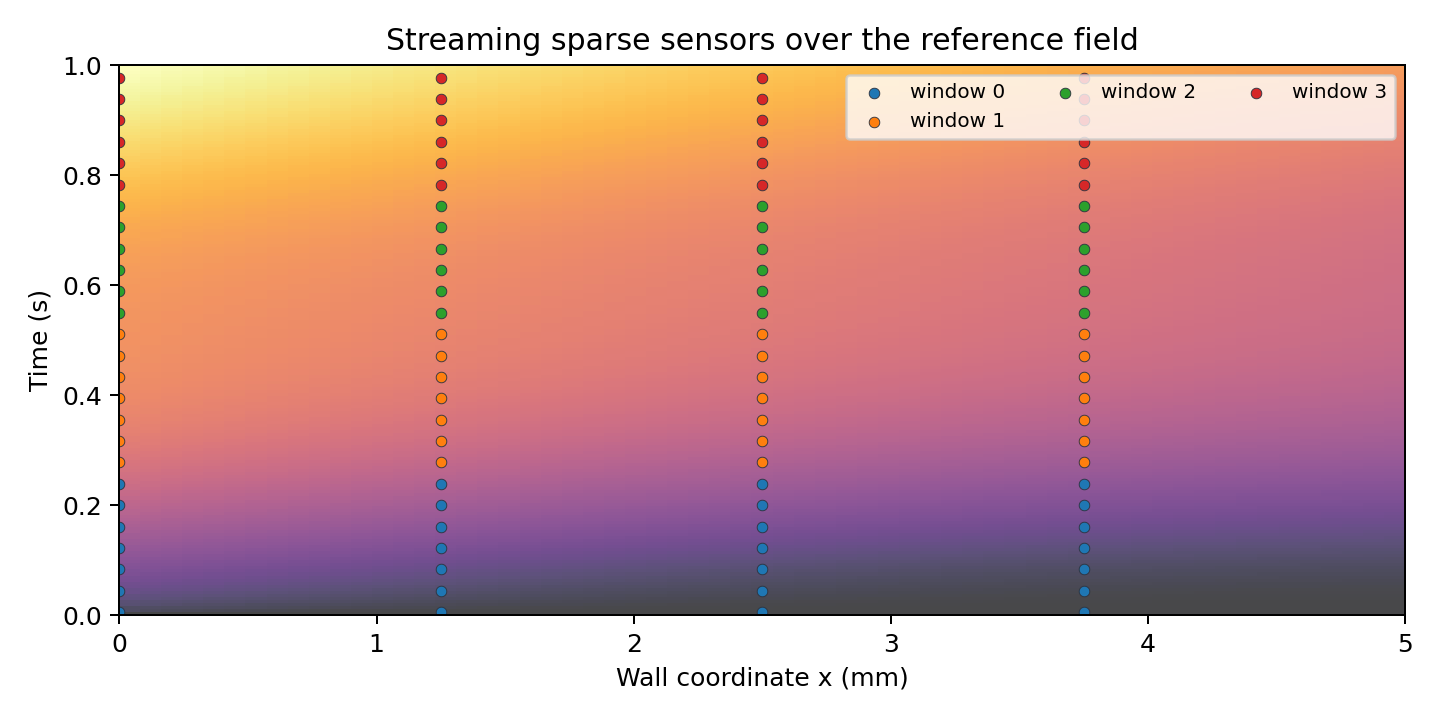
\includegraphics[width=0.82\linewidth]{figures/sensor_streaming_map.png}
    \caption{Sparse thermocouple-like observations used by the adaptive PINN. The windows are sequential time batches, not moving physical boundaries. After each batch arrives, the model is fine-tuned using the accumulated sensor observations.}
    \label{fig:sensors}
\end{figure}

The adaptive model starts from the baseline PINN weights. When sensor window $m$ arrives, the model is fine-tuned with
\begin{equation}
\mathcal{L}_{\mathrm{adaptive}}
= \mathcal{L}_{\mathrm{base}}
+ w_{\mathrm{sensor}}\mathcal{L}_{\mathrm{sensor}},
\end{equation}
where
\begin{equation}
\mathcal{L}_{\mathrm{sensor}}
= \frac{1}{N_s}\sum_{j=1}^{N_s}
\left[
\theta_\mathrm{PINN}(\hat{x}_j,\hat{t}_j)
- \theta^{\mathrm{sensor}}_j
\right]^2 .
\end{equation}
This makes the project comparison very direct: the architecture and governing equation are the same, but the adaptive model receives sparse sensor observations after the offline baseline is trained.

\section{Preliminary Results}
Figure~\ref{fig:summary} summarizes the three-seed preliminary study. The adaptive model consistently improves both the global relative $L_2$ error and the hot-side maximum error. The hot side is especially important because it corresponds to the surface exposed to the rocket hot-gas heat flux.

\begin{figure}[h!]
    \centering
    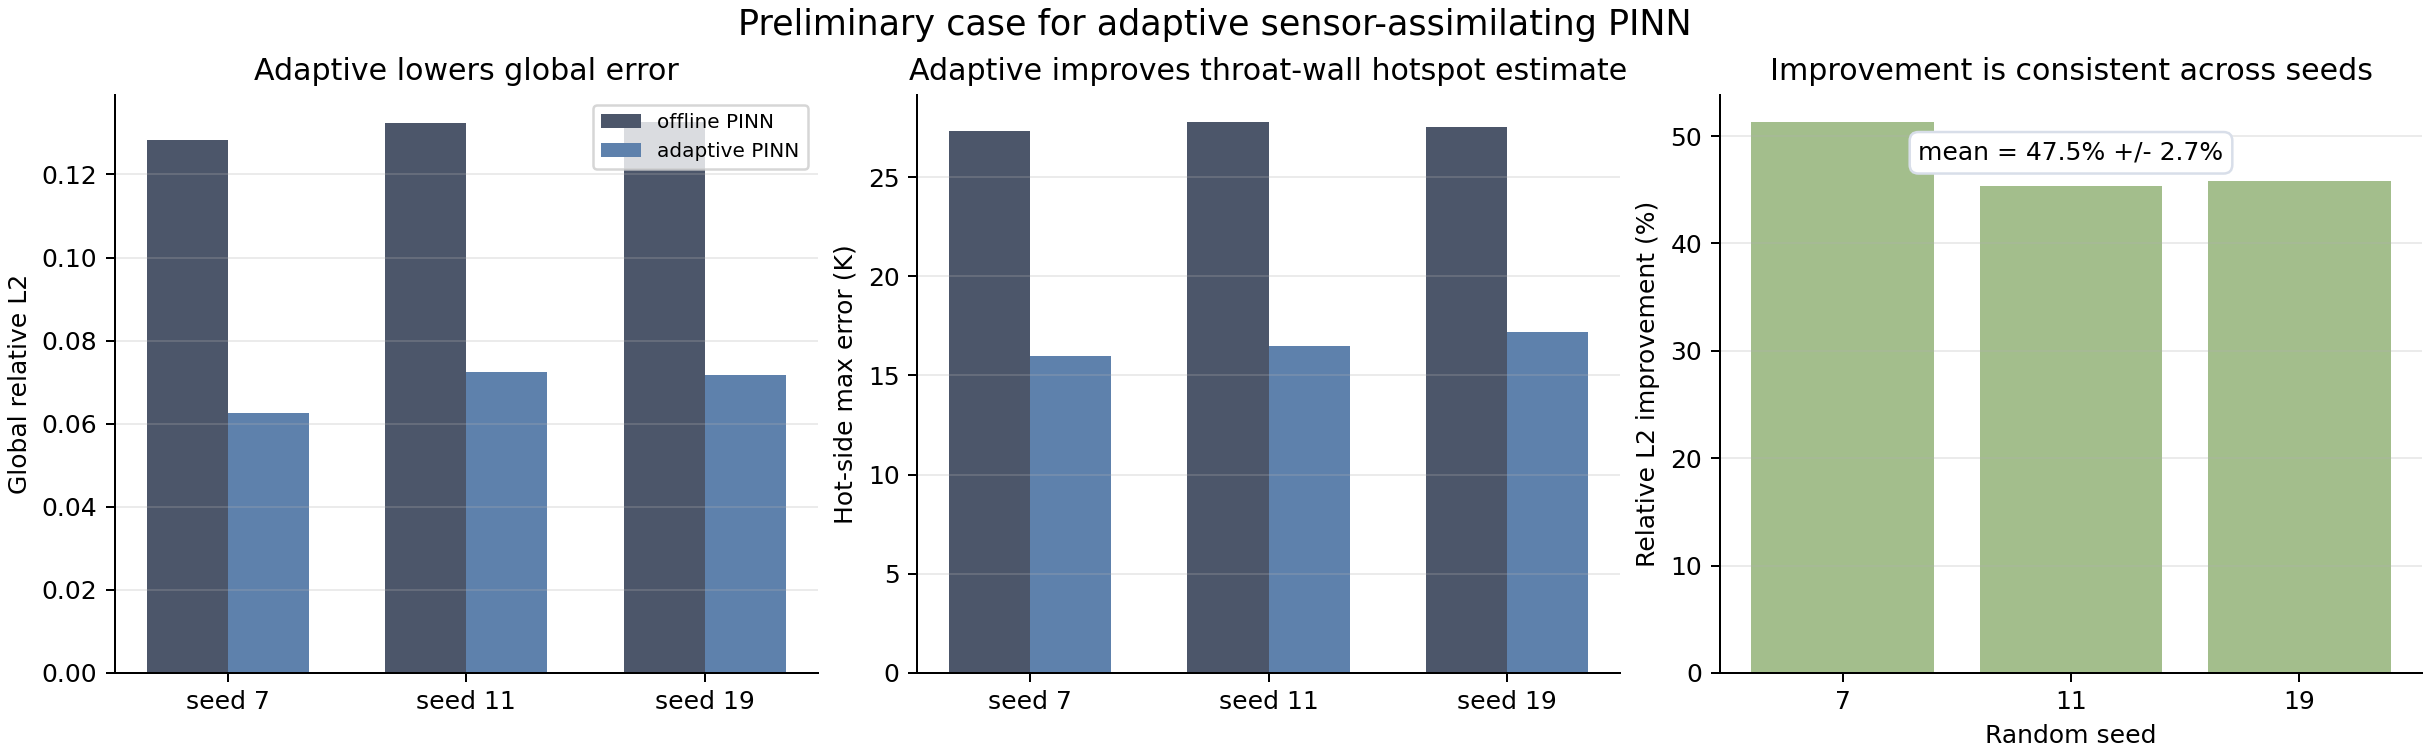
\includegraphics[width=0.98\linewidth]{figures/case_summary.png}
    \caption{Preliminary multi-seed comparison. The adaptive PINN improves the global relative $L_2$ error and the hot-side maximum temperature error across all tested seeds.}
    \label{fig:summary}
\end{figure}

\begin{table}[h!]
\centering
\caption{Three-seed preliminary metrics for the PyTorch implementation.}
\label{tab:metrics}
\begin{tabular}{lcc}
\toprule
Metric & Offline PINN & Adaptive PINN \\
\midrule
Global relative $L_2$ error & $0.1312 \pm 0.0019$ & $0.0689 \pm 0.0045$ \\
Hot-side maximum error [K] & $27.53 \pm 0.19$ & $16.56 \pm 0.49$ \\
\bottomrule
\end{tabular}
\end{table}

Figure~\ref{fig:error} gives a more detailed visual comparison for one representative seed. The right panel shows the change in absolute error. Positive regions indicate where the adaptive model reduced the error compared with the offline baseline.

\begin{figure}[h!]
    \centering
    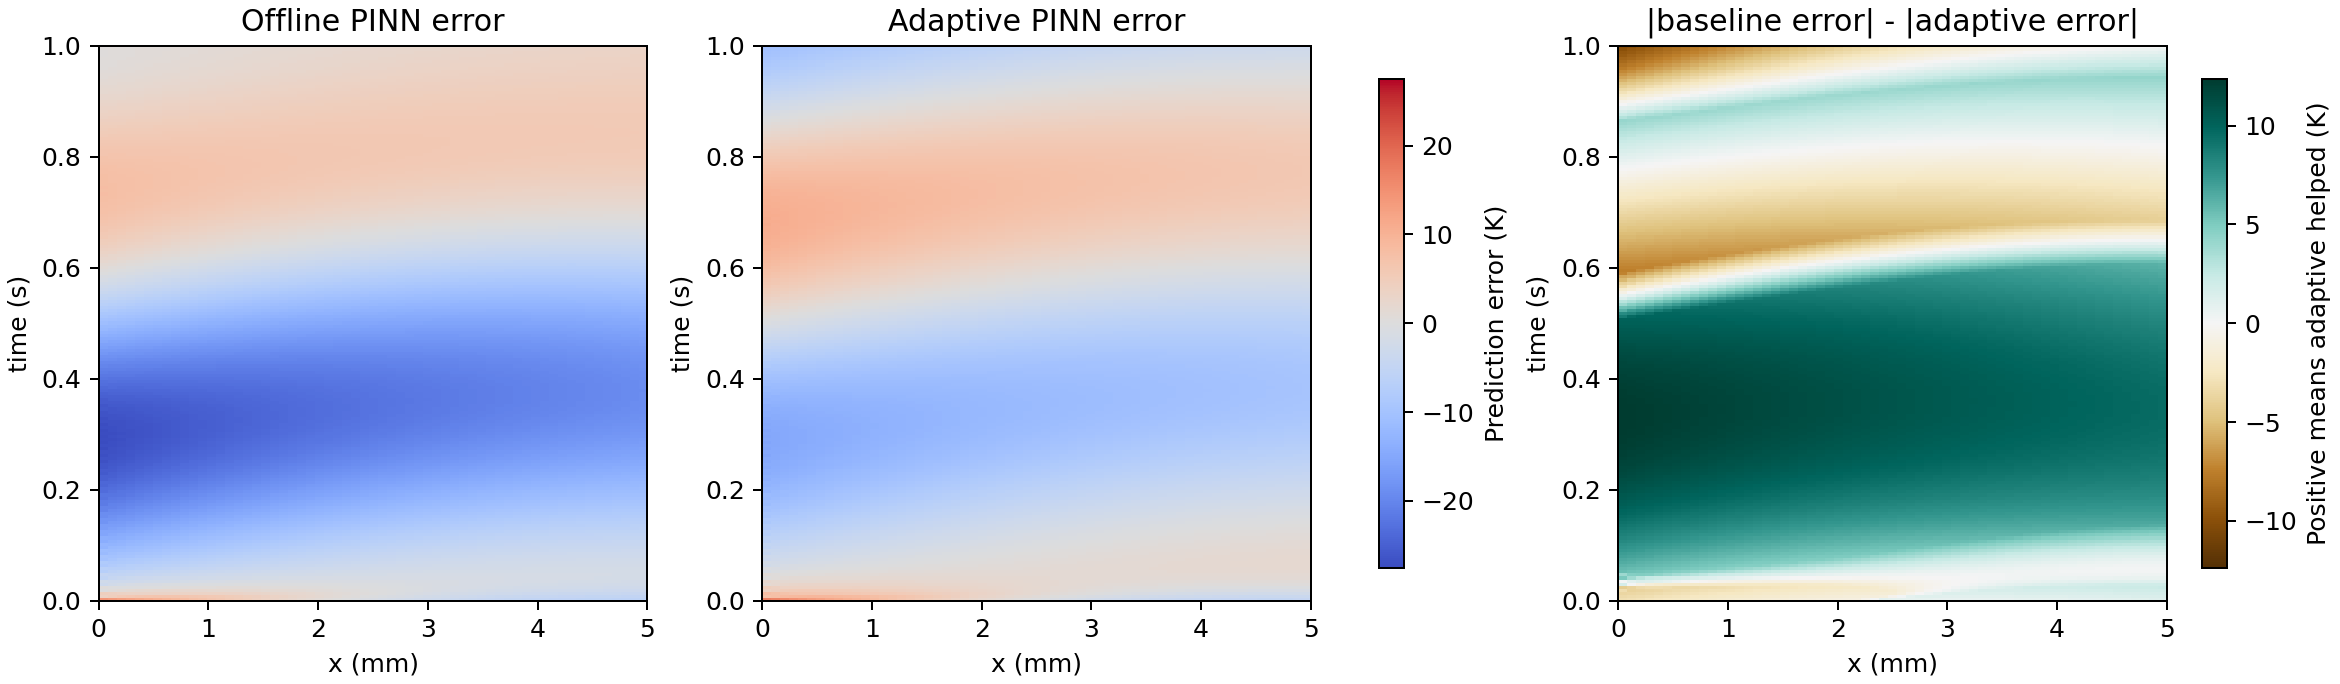
\includegraphics[width=0.98\linewidth]{figures/error_heatmaps.png}
    \caption{Representative error fields for the offline and adaptive PINNs. The adaptive model reduces error in most of the space--time domain, especially near the hot side after sensor information is assimilated.}
    \label{fig:error}
\end{figure}

\section{Remaining Work}
The current code already reaches the course milestone of a runnable baseline and one controlled modification. The next two weeks will focus on making the final comparison more rigorous:
\begin{enumerate}
    \item run the full experiment with more epochs and a finer grid for final-quality figures;
    \item test sensitivity to sensor noise, sensor placement, and sensor-loss weight;
    \item report cases where adaptive updates help globally but may locally hurt unobserved regions;
    \item convert this preliminary report into the final AIAA manuscript format with a concise results and limitations discussion.
\end{enumerate}

The fallback plan is to keep the project as a controlled robustness study. If adaptive updates do not always improve the result, that is still scientifically meaningful: it would show when sparse sensor assimilation helps and when it conflicts with the physics loss or boundary conditions.

\begin{thebibliography}{9}

\bibitem{oates1984aerothermodynamics}
Oates, G. C., ed., \textit{Aerothermodynamics of Gas Turbine and Rocket Propulsion}, AIAA Education Series, American Institute of Aeronautics and Astronautics, New York, 1984.

\bibitem{patankar1980numerical}
Patankar, S. V., \textit{Numerical Heat Transfer and Fluid Flow}, Hemisphere Publishing Corporation, 1980.

\bibitem{raissi2019pinn}
Raissi, M., Perdikaris, P., and Karniadakis, G. E., ``Physics-informed neural networks: A deep learning framework for solving forward and inverse problems involving nonlinear partial differential equations,'' \textit{Journal of Computational Physics}, Vol. 378, 2019, pp. 686--707. doi:10.1016/j.jcp.2018.10.045.

\bibitem{cai2021heat}
Cai, S., Wang, Z., Wang, S., Perdikaris, P., and Karniadakis, G. E., ``Physics-Informed Neural Networks for Heat Transfer Problems,'' \textit{Journal of Heat Transfer}, Vol. 143, No. 6, 2021, 060801. doi:10.1115/1.4050542.

\end{thebibliography}

\end{document}
